\documentclass[12pt]{article}
\usepackage{fullpage}
\usepackage{hyperref}
\hypersetup{bookmarks=true,colorlinks=true,linkcolor=red,citecolor=blue,filecolor=magenta,urlcolor=cyan}
\usepackage{amsmath}
\usepackage{longtable}
\usepackage{booktabs}
\usepackage{caption}
\usepackage{graphics}
\title{Software Requirements Specification for Slope Stability Analysis}
\author{Henry Frankis}
\begin{document}
\maketitle
\tableofcontents
\newpage
\section{Reference Material}
\label{Sec:RM}
\subsection{Table of Units}
\label{Sec:ToU}
Units of the physical properties of the soil that are of interest when examining slope stability problems are given in the following table.
\begin{longtable}{l l l}
\toprule
Symbol & Description & Name
\\
\midrule
m & length & Metre
\\
${}^{\circ}$ & angle & Degree
\\
N & force & Newton
\\
Pa & pressure & Pascal
\\
\bottomrule
\caption{Table of Units}
\label{Table:ToU}
\end{longtable}
\subsection{Table of Symbols}
\label{Sec:ToS}
A collection of the symbols that will be used in the models and equations of the program are summarized in the table below. Values with a subscript i implies that the value will be taken at and analyzed at a slice or slice interface composing the total slip mass.
\begin{longtable*}{l l l}
\toprule
Symbol & Units & Description
\\
\midrule
$\varphi{}'$ & ${}^{\circ}$ & effective angle of friction
\\
$c'$ & Pa & effective cohesion
\\
$\gamma{}$ & $\frac{\text{N}}{\text{m}^{3}}$ & unit weight of dry soil/ground layer
\\
$\gamma{}_{Sat}$ & $\frac{\text{N}}{\text{m}^{3}}$ & unit weight of saturated soil/ground layer
\\
$\gamma{}_{w}$ & $\frac{\text{N}}{\text{m}^{3}}$ & unit weight of water
\\
$E$ & Pa & elastic modulus
\\
$\nu{}$ & unitless & Poisson's ratio
\\
$(x,y)$ & m & cartesian position coordinates; y is considered parallel to the direction of the force of gravity and x is considered perpendicular to y
\\
$y_{wt,i}$ & m & the y ordinate, or height of the water table at i; refers to either slice i midpoint, or slice interface i
\\
$y_{us,i}$ & m & the y ordinate, or height of the top of the slope at i; refers to either slice i midpoint, or slice interface i
\\
$y_{slip,i}$ & m & the y ordinate, or height of the slip surface at i; refers to either slice i midpoint, or slice interface i
\\
$x_{i}$ & m & the x ordinate; refers to either slice i midpoint, or slice interface i
\\
$({x_{cs}},{y_{cs}})$ & m & the set of x and y coordinates that describe the vertices of the critical slip surface
\\
$FS$ & unitless & global factor of safety describing the stability of a surface in a slope
\\
$FS_{Loc,i}$ & unitless & local factor of safety specific to a slice i
\\
$S_{i}$ & N & mobilized shear force for slice i
\\
$P_{i}$ & N & shear resistance; Mohr Coulomb frictional force that describes the limit of mobilized shear force the slice i can withstand before failure
\\
$T_{i}$ & N & mobilized shear force without the influence of interslice forces for slice i
\\
$R_{i}$ & N & shear resistance without the influence of interslice forces for slice i
\\
$W_{i}$ & N & weight; downward force caused by gravity on slice i
\\
$K_{c}$ & unitless & earthquake load factor; proportionality factor of force that weight pushes outwards; caused by seismic earth movements
\\
$H_{i}$ & N & interslice water force exerted in the x-ordinate direction between adjacent slices (for interslice index i)
\\
$\Delta{}H_{i}$ & N & difference between interslice forces on acting in the x-ordinate direction of the slice on each side (for interslice index i)
\\
$E_{i}$ & N & interslice normal force being exerted between adjacent slices (for interslice index i)
\\
$X_{i}$ & N & interslice shear force being exerted between adjacent slices (for interslice index i)
\\
$U_{b,i}$ & N & base hydrostatic force arising from water pressure within the slice (for slice index i)
\\
$U_{t,i}$ & N & surface hydrostatic force arising from water pressure acting into the slice from standing water on the slope surface (for slice index i)
\\
$N_{i}$ & N & total reactive force for a soil surface subject to a body resting on it
\\
$N'_{i}$ & N & effective normal force of a soil surface, subtracting pore water reactive force from total reactive force
\\
$N*_{i}$ & N & effective normal force of a soil surface, neglecting the influence of interslice forces
\\
$Q_{i}$ & N & imposed surface load; a downward force acting into the surface from midpoint of slice i
\\
$\alpha{}_{i}$ & ${}^{\circ}$ & angle of the base of the mass relative to the horizontal (for slice index i)
\\
$\beta{}_{i}$ & ${}^{\circ}$ & angle of the surface of the mass relative to the horizontal (for slice index i)
\\
$\omega{}_{i}$ & ${}^{\circ}$ & angle of imposed surface load acting into the surface relative to the vertical (for slice index i)
\\
$\lambda{}$ & unitless & ratio between interslice normal and shear forces (applied to all interslices)
\\
$f_{i}$ & unitless & scaling function for magnitude of interslice forces as a function of the x coordinate (at interslice index i); can be constant or a half-sine
\\
$b_{i}$ & m & base width of the slice in the x-ordinate direction only (for slice index i)
\\
$\ell{}_{b,i}$ & m & total length of the base of a slice (for slice index i)
\\
$\ell{}_{s,i}$ & m & length of an interslice surface, from slip base to slope surface in a vertical line from an interslice vertex (for interslice index i)
\\
$h_{i}$ & m & midpoint height; distance from the slip base to the slope surface in a vertical line from the midpoint of the slice (for slice i)
\\
$n$ & unitless & number of slices the slip mass has been divided into
\\
$F$ & m & generic force; assumed 1D allowing a scalar
\\
$M$ & Nm & moment of a body; assumed 2D allowing a scalar
\\
$\Upsilon{}$ & unitless & generic minimization function or algorithm
\\
$\delta{}$ & m & generic displacement of a body
\\
$K$ & $\frac{\text{N}}{\text{m}}$ & stiffness (how much a body resists displacement when subject to a force)
\\
$K_{st,i}$ & Pa & shear stiffness of an interslice surface, without length adjustment (for interslice index i)
\\
$K_{bt,i}$ & Pa & shear stiffness of a slice base surface, without length adjustment (for slice index i)
\\
$K_{sn,i}$ & Pa & normal stiffness of an interslice surface, without length adjustment (for interslice index i)
\\
$K_{bn,i}$ & Pa & normal stiffness of a slice base surface, without length adjustment (for slice index i)
\\
$K_{tr}$ & Pa & residual shear stiffness
\\
$K_{no}$ & Pa & residual normal stiffness
\\
$\delta{}u_{i}$ & m & shear displacement of a slice (for slice index i)
\\
$\delta{}v_{i}$ & m & normal displacement of a slice (for slice index i)
\\
$\delta{}x_{i}$ & m & displacement of a slice in the x-ordinate direction (for slice index i)
\\
$\delta{}y_{i}$ & m & displacement of a slice in the y-ordinate direction (for slice index i)
\\
\bottomrule
\label{Table:ToS}
\end{longtable*}
\subsection{Abbreviations and Acronyms}
\label{Sec:AaA}
\begin{longtable*}{l l}
\toprule
Symbol & Description
\\
\midrule
A & Assumption
\\
DD & Data Definition
\\
GD & General Definition
\\
GS & Goal Statement
\\
IM & Instance Model
\\
LC & Likely Change
\\
PS & Physical System Description
\\
R & Requirement
\\
SRS & Software Requirements Specification
\\
SSA & Slope Stability Analysis
\\
T & Theoretical Model
\\
\bottomrule
\label{Table:AaA}
\end{longtable*}
\section{Introduction}
\label{Sec:I}
A slope of geological mass, composed of soil and rock, is subject to the influence of gravity on the mass. For an unstable slope this can cause instability in the form of soil/rock movement. The effects of soil/rock movement can range from inconvenient to seriously hazardous, resulting in signifcant life and economic loses. Slope stability is of interest both when analyzing natural slopes, and when designing an excavated slope. Slope stability analysis is the assessment of the safety of a slope, identifying the surface most likely to experience slip and an index of it's relative stability known as the factor of safety.
The following section provides an overview of the Software Requirements Specification (SRS) for a slope stability analysis problem. The developed program will be referred to as the Slope Stability Analysis (SSA) program. This section explains the purpose of this document, the scope of the system, the organization of the document and the characteristics of the intended readers.
\subsection{Purpose}
\label{Sec:P}
The SSA program determines the critical slip surface, and it's respective factor of safety as a method of assessing the stability of a slope design. The program is intended to be used as an educational tool for introducing slope stability issues, and will facilitate the analysis and design of a safe slope.
This document will be used as a starting point for subsequent development phases, including writing the design specification and the software verification and validation plan.  The design document will show how the requirements are to be realized, including decisions on the numerical algorithms and programming environment.  The verification and validation plan will show the steps that will be used to increase confidence in the software documentation and the implementation.  Although the SRS fits in a series of documents that follow the so-called waterfall model, the actual development process is not  constrained in any way.  Even when the waterfall model is not followed, as Parnas and Clements point out, the most logical way to present the documentation is still to fake a rational design process.
\subsection{Scope of Requirements}
\label{Sec:SoR}
The scope of the requirements is limited to stability analysis of a 2 dimensional slope, composed of homogeneous soil layers. Given appropriate inputs, the code for SSA will identify the most likely failure surface within the possible input range, and find the factor of safety for the slope as well as displacement of soil that will occur on the slope.
\subsection{Organization of Document}
\label{Sec:OoD}
The organization of this document follows the template for an SRS for scientific computing software proposed by Koothoor as well as Smith and Lai.  The presentation follows the standard pattern of presenting goals, theories, definitions, and assumptions.  For readers that would like a more bottom up approach, they can start reading the instance models in Section~\ref{Sec:IM} and trace back to find any additional information they require.  The instance models provide the set of algebraic equations that must be solved iteratively to perform a Morgenstern Price Analysis. The goal statements are refined to the theoretical models (Section~\ref{Sec:TM}) and instance models (Section~\ref{Sec:IM}).
\section{General System Description}
\label{Sec:GSD}
This section provides general information about the system, identifies the interfaces between the system and its environment, and describes the user characteristics and the system constraints.
\subsection{User Characteristics}
\label{Sec:UC}
The end user of SSA should have an understanding of undergraduate Level 1 Calculus and Physics, and be familiar with soil and material properties.
\subsection{System Constraints}
\label{Sec:SC}
There are no system constraints.
\section{Specific System Description}
\label{Sec:SSD}
This section first presents the problem description, which gives a high-level view of the problem to be solved.  This is followed by the solution characteristics specification, which presents the assumptions, theories, definitions and finally the instance models that model the slope.
\subsection{Problem Description}
\label{Sec:PD}
SSA is a computer program developed to evaluate the factor of safety of a slopes slip surface and to calculate the displacement that the slope will experience.
\subsubsection{Terminology}
\label{Sec:T}
\begin{itemize}
\item[Factor of Safety:]Stability metric. How likely a slip surface is to experience failure through slipping.
\item[Critical Slip Surface:]Slip surface of the slope that has the lowest global factor of safety, and therefore most likely to experience failure.
\item[Stress:]Forces that are exerted between planes internal to a larger body subject to external loading.
\item[Strain:]Stress forces that result in deformation of the body/plane.
\item[Normal Force:]A force applied perpendicular to the plane of the material.
\item[Shear Force:]A force applied parallel to the plane of the material.
\item[Tension:]A stress the causes displacement of the body away from it's center.
\item[Compression:]A stress the causes displacement of the body towards it's center.
\item[Plane Strain:]The resultant stresses in one of the directions of a 3 dimensional material can be approximated as 0. Results when the length of one dimension of the body dominates the others. Stresses in the dominate dimensions direction are the ones that can be approximated as 0.
\end{itemize}
\subsubsection{Physical System Description}
\label{Sec:PSD}
Analysis of the slope is performed by looking at properties of the slope as a series of slice elements. Some properties are interslice properties, and some are slice or slice base properties.  The index convention for referencing which interslice or slice is being used is shown in Figure~\ref{Figure:Icfnsaifv}.
\begin{enumerate}
\item{Interslice properties convention is noted by j. The end interslice properties are usually not of interest, therefore use the interslice properties from 1 $\leq{}$ i $\leq{}$ n-1.}
\item{Slice properties convention is noted by i.}
\end{enumerate}
A free body diagram of the forces acting on the slice is displayed in Figure~\ref{Figure:Faoas}.
\begin{figure}
\begin{center}
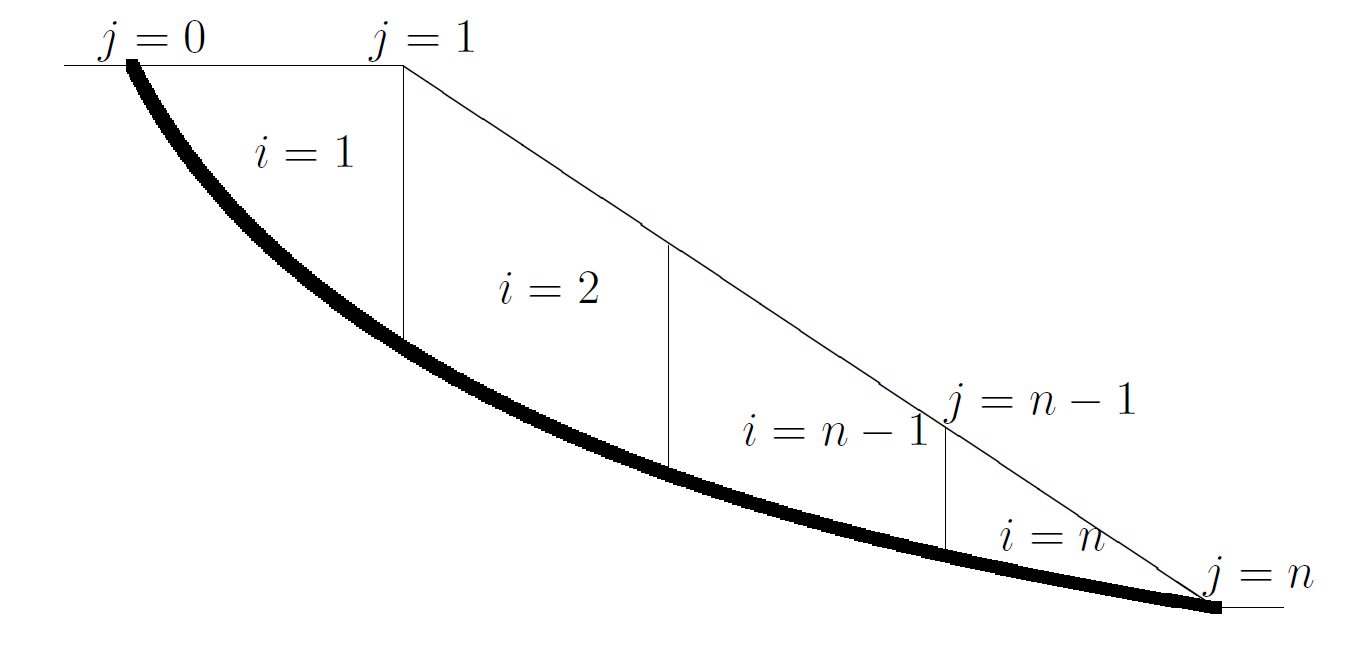
\includegraphics{IndexConvention.png}
\caption{Index convention for numbering slice and interslice force variables}
\label{Figure:Icfnsaifv}
\end{center}
\end{figure}
\begin{figure}
\begin{center}
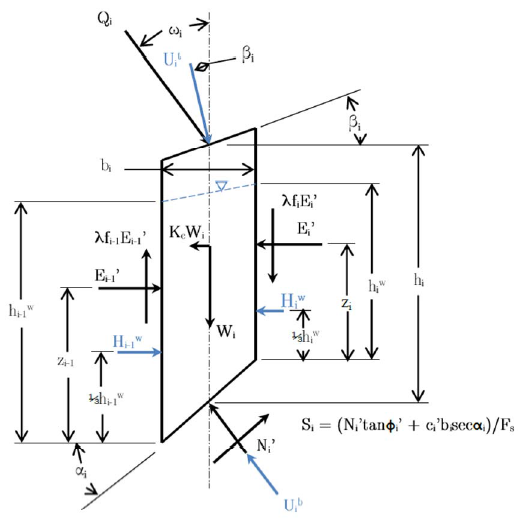
\includegraphics{ForceDiagram.png}
\caption{Forces acting on a slice}
\label{Figure:Faoas}
\end{center}
\end{figure}
\subsubsection{Goal Statements}
\label{Sec:GS}
Given the geometry of the water table, the geometry of the layers composing the plane of a slope, and the material properties of the layers.
\begin{itemize}
\item[GS1:]Evaluate local and global factors of safety along a given slip surface.
\item[GS2:]Identify the critical slip surface for the slope, with the lowest Factor of Safety.
\item[GS3:]Determine the displacement of the slope.
\end{itemize}
\subsection{Solution Characteristics Specification}
\label{Sec:SCS}
The instance models that govern SSA are presented in Section~\ref{Sec:IM}.  The information to understand the meaning of the instance models and their derivation is also presented, so that the instance models can be verified.
\subsubsection{Assumptions}
\label{Sec:A}
This section simplifies the original problem and helps in developing the theoretical model by filling in the missing information for the physical system. The numbers given in the square brackets refer to the data definition, or the instance model, in which the respective assumption is used.
\begin{itemize}
\item[A1:]The slip surface is concave with respect to the slope surface. The $(x,y)$ coordinates of the failure surface follow a monotonic function.
\item[A2:]The geometry of the slope, and the material properties of the soil layers are given as inputs.
\item[A3:]The different layers of the soil are homogeneous, with consistent soil properties throughout, and independent of dry or saturated conditions, with the exception of unit weight.
\item[A4:]Soil layers are treated as if they have isotropic properties.
\item[A5:]Interslice normal and shear forces have a linear relationship, proportional to a constant ($\lambda{}$) and an interslice force function ($f_{i}$) depending on x position.
\item[A6:]Slice to base normal and shear forces have a linear relationship, dependent on the factor of safety ($FS$), and the Coulomb sliding law.
\item[A7:]The stress-strain curve for interslice relationships is linear with a constant slope.
\item[A8:]The slope and slip surface extends far into and out of the geometry (z coordinate). This implies plane strain conditions, making 2D analysis appropriate.
\item[A9:]The effective normal stress is large enough that the resistive shear to effective normal stress relationship can be approximated as a linear relationship.
\item[A10:]The surface and base of a slice between interslice nodes are approximated as straight lines.
\end{itemize}
\subsubsection{Theoretical Models}
\label{Sec:TM}
This section focuses on the general equations and laws that SSA is based on.
~\newline
\noindent \begin{minipage}{\textwidth}
\begin{tabular}{p{0.2\textwidth} p{0.73\textwidth}}
\toprule \textbf{Refname} & \textbf{T:FoS}
\phantomsection 
\label{T:FoS}
\\ \midrule \\
Label & Factor of Safety
\\ \midrule \\
Equation & $FS=\frac{P}{S}$
\\ \midrule \\
Description & The stability metric of the slope, known as the factor of safety ($FS$), is determined by the ratio of the shear force at the base of the slope ($S$), and the resistive shear ($P$).
\\ \bottomrule \end{tabular}
\end{minipage}\\
\subsubsection{General Definitions}
\label{Sec:GD}
\subsubsection{Data Definitions}
\label{Sec:DD}
\subsubsection{Instance Models}
\label{Sec:IM}
\subsubsection{Data Constraints}
\label{Sec:DC}
\section{Requirements}
\label{Sec:R}
This section provides the functional requirements, the business tasks that the software is expected to complete, and the nonfunctional requirements, the qualities that the software is expected to exhibit.
\subsection{Functional Requirements}
\label{Sec:FR}
\begin{itemize}
\item[R1:]Read the input file, and store the data. Necessary input data summarized in Table~\ref{Table:Id}.
\item[R2:]Generate potential critical slip surface's for the input slope.
\item[R3:]Test the slip surfaces to determine if they are physically realizable based on a set of pass or fail criteria.
\item[R4:]Prepare the slip surfaces for a method of slices or limit equilibrium analysis.
\item[R5:]Calculate the factors of safety of the slip surfaces.
\item[R6:]Rank and weight the slopes based on their factor of safety, such that a slip surface with a smaller factor of safety has a larger weighting.
\item[R7:]Generate new potential critical slip surfaces based on previously analysed slip surfaces with low factors of safety.
\item[R8:]Repeat requirements R3 to R7 until the minimum factor of safety remains approximately the same over a predetermined number of repetitions. Identify the slip surface that generates the minimum factor of safety as the critical slip surface.
\item[R9:]Prepare the critical slip surface for method of slices or limit equilibrium analysis.
\item[R10:]Calculate the factor of safety of the critical slip surface using the Morgenstern price method.
\item[R11:]Display the critical slip surface and the slice element displacements graphically. Give the values of the factors of safety calculated by the Morgenstern price method.
\end{itemize}
\begin{longtable}{l l l}
\toprule
Symbol & Units & Description
\\
\midrule
$(x,y)$ & m & cartesian position coordinates; y is considered parallel to the direction of the force of gravity and x is considered perpendicular to y
\\
$E$ & Pa & elastic modulus
\\
$c'$ & Pa & effective cohesion
\\
$\nu{}$ & unitless & Poisson's ratio
\\
$\varphi{}'$ & ${}^{\circ}$ & effective angle of friction
\\
$\gamma{}$ & $\frac{\text{N}}{\text{m}^{3}}$ & unit weight of dry soil/ground layer
\\
$\gamma{}_{Sat}$ & $\frac{\text{N}}{\text{m}^{3}}$ & unit weight of saturated soil/ground layer
\\
$\gamma{}_{w}$ & $\frac{\text{N}}{\text{m}^{3}}$ & unit weight of water
\\
\bottomrule
\caption{Input data}
\label{Table:Id}
\end{longtable}
\subsection{Nonfunctional Requirements}
\label{Sec:NR}
SSA is intended to be an educational tool, therefore accuracy and performance speed are secondary program priorities to correctness, understandability, reusability, and maintainability.
\section{Likely Changes}
\label{Sec:LC}
\end{document}
